% Retoca las líneas marcadas con TODO según las necesidades

\documentclass[oneside,a4paper,12pt]{book} % TODO: cambia "oneside" por "twoside" a la hora de imprimirlo

\usepackage[spanish]{babel}
\usepackage[utf8]{inputenc}
\usepackage{geometry}
\usepackage{makeidx}
\usepackage{url}
\usepackage{graphicx}
\usepackage{color}
\usepackage{caption}
\usepackage{acronym}
\usepackage{hyphenat}
\usepackage{a4wide}
\usepackage[normalsize]{subfigure}
\usepackage{float}
\usepackage{titlesec}
\usepackage[Lenny]{fncychap}
\usepackage{listings} % para poder hacer uso de "listings" propios (p.ej. códigos)
\usepackage{eurosym} % para poder usar el símbolo del euro con \euro {xx}
\usepackage{hyperref} % TODO: añade la opción hidelinks para imprimirlo (los enlaces no aparecerán resaltados)

% Para que no parta las palabras
\pretolerance=10000

\newcommand{\bigrule}{\titlerule[0.5mm]} \titleformat{\chapter}[display] % cambiamos el formato de los capítulos
{\bfseries\Huge} % por defecto se usaron caracteres de tamaño huge en negrita
{% contenido de la etiqueta 
\titlerule % línea horizontal 
\filright % texto alineado a la derecha 
\Large\chaptertitlename\ % capítulo e índice en tamaño large
\Large % en lugar de 
\Huge \Large\thechapter} 
{0mm} % espacio mínimo entre etiqueta y cuerpo
{\filright} % texto del cuerpo alineado a la derecha
[\vspace{0.5mm} \bigrule] % después del cuerpo, dejar espacio vertical y trazar línea horizontal gruesa
\geometry{a4paper, left=3.5cm, right=2cm, top=3cm, bottom=2cm, headsep=1.5cm}

% Estilos para ilustrar códigos:
\definecolor{code_green}{rgb}{0,0.6,0}
\definecolor{code_gray}{rgb}{0.5,0.5,0.5}
\definecolor{code_mauve}{rgb}{0.58,0,0.82}

\lstset{frame=tb,
  language=C,
  aboveskip=3mm,
  belowskip=3mm,
  showstringspaces=false,
  columns=flexible,
  basicstyle={\small\ttfamily},
  numbers=none,
  numberstyle=\tiny\color{code_gray},
  keywordstyle=\color{blue},
  commentstyle=\color{code_green},
  stringstyle=\color{code_mauve},
  breaklines=true,
  breakatwhitespace=true,
  tabsize=3
}

\lstset{frame=tb,
  language=C++,
  aboveskip=3mm,
  belowskip=3mm,
  showstringspaces=false,
  columns=flexible,
  basicstyle={\small\ttfamily},
  numbers=none,
  numberstyle=\tiny\color{code_gray},
  keywordstyle=\color{blue},
  commentstyle=\color{code_green},
  stringstyle=\color{code_mauve},
  breaklines=true,
  breakatwhitespace=true,
  tabsize=3
}

\lstset{frame=tb,
  language=Python,
  aboveskip=3mm,
  belowskip=3mm,
  showstringspaces=false,
  columns=flexible,
  basicstyle={\small\ttfamily},
  numbers=none,
  numberstyle=\tiny\color{code_gray},
  keywordstyle=\color{blue},
  commentstyle=\color{code_green},
  stringstyle=\color{code_mauve},
  breaklines=true,
  breakatwhitespace=true,
  tabsize=3
}

% Definición de mis propios tipos: Códigos, Ecuaciones y Tablas
\DeclareCaptionType{code}[Código][Listado de códigos]
\DeclareCaptionType{myequation}[Ecuación][Listado de ecuaciones]

% TODO: especifica las reglas de separación que consideres. Algunos ejemplos:
\hyphenation{fuer-tes}
\hyphenation{mul-ti-ca-pa}
\hyphenation{res-pues-ta}
\hyphenation{di-fe-ren-tes}
\hyphenation{de-sa-rro-lla-dos}
\hyphenation{re-pre-sen-tan-do}

 % archivo de configuraci�n de estilo

\makeindex

\begin{document}
\baselineskip 1.35\baselineskip

\frontmatter

\thispagestyle{empty}
\vspace{2cm}

\begin{figure}[htb]
  \centerline{\resizebox{.60\textwidth}{!}{\includegraphics{figs/logo_urjc}}}
\end{figure}

\begin{center}
  {\Large {\bf GRADO EN INGENIERÍA DE ROBÓTICA SOFTWARE}}
  \vspace{5mm}
 
  {\large {Escuela de Ingeniería de Fuenlabrada}}
  \vspace{5mm}

  {\large {Curso académico 2023-2024}}

  \vspace{1cm}

  {\large {\bf Trabajo Fin de Grado}}

  \vspace{2cm}

  {\Large {Brazo robótico de bajo coste para la docencia universitaria  \\[1cm] }}

  \vspace{5cm}
  {\bf Tutor}: Julio Vega Pérez \\
  {\bf Autor}: Vidal Pérez Bohoyo
\end{center}

\clearpage
\thispagestyle{empty}


% Este diseño se corresponde con la licencia CC-BY-NC-SA.
% Por supuesto, puedes poner la licencia que mejor se adapte al propósito de tu trabajo.
% Recuerda que, si no se especifica ninguna licencia, esta -como cualquier creación artística- pasaría a estar licenciada con todos los derechos reservados (copyright).

\vspace{5cm}

\begin{flushright}

\begin{figure}
\includegraphics[width=0.10\textwidth,right]{figs/by-nc-sa.png}
\end{figure}

\vspace{0.2cm}

{\tiny 
(CC) \textbf{Vidal Pérez Bohoyo}\\ % TODO: pon aquí tu nombre cuando hagas el documento
\vspace{0.5cm}
\emph{
Este trabajo se entrega bajo licencia \href{https://creativecommons.org/licenses/by-nc-sa/3.0/es/}{CC BY-NC-SA}. \\
Usted es libre de \textit{(a) compartir}: copiar y redistribuir el material en \\
cualquier medio o formato; y \textit{(b) adaptar}: remezclar, transformar \\
y crear a partir del material. El licenciador no puede revocar estas \\
libertades mientras cumpla con los términos de la licencia. \\}
}

\end{flushright}



\cleardoublepage

\chapter*{Agradecimientos}

\noindent En primer lugar, quiero agradecer a mi profesor guía, Julio Vega, por su apoyo y orientación a lo largo de este trabajo. Sus conocimientos y 
sugerencias fueron de gran ayuda para enfocarlo adecuadamente y alcanzar resultados significativos.

A mi familia, gracias por su apoyo incondicional y por creer en mí en cada paso de mi formación académica. En espacial a mi primo Pablo, que desde 
pequeño me ha introducido en el mundo de la ingeniería y siempre ha estado ahí cuando más lo he necesitado.

A mi novia, por compartir este viaje conmigo y haberme levantado tras cada caída. Su compañía y paciencia me ha hecho lograr lo que en un momento pensé 
que era imposible. Gracias por ser y haber sido un pilar fundamental en mi vida.

Agradezco también a todas las personas que participaron en la investigación, brindando su tiempo y conocimientos. Como ha sido el caso de Julio Salvador 
Lora.

Por último, quiero agradecer a todas las personas que, de alguna manera, me han apoyado durante este proceso, incluso si no están mencionadas 
específicamente. Sus palabras de apoyo y sus consejos me han motivado aún más en este proyecto.

Este logro es el resultado de un esfuerzo conjunto, y agradezco sinceramente a cada persona que ha sido parte de él. Espero que este 
trabajo contribuya al desarrollo de la robótica y que pueda inspirar futuras investigaciones.

\ % Algo de separación...

\

\

\

\

\begin{flushright}
		\vspace{4.0 cm}
		\emph{A mi familia y a mi novia.}\\
		\par
		\vspace{1.0 cm}
		Madrid, 11 de octubre de 2023\\ %\today
		\emph{Vidal Pérez Bohoyo}
\end{flushright}

\thispagestyle{empty}



\cleardoublepage

\chapter*{Resumen\markboth{Resumen}{Resumen}}
\noindent La robótica ---disciplina enfocada en el diseño, construcción y programación de robots--- se compone de 
diversas ramas entre las cuales interesa destacar la robótica educativa, caracterizada por 
ofrecer robots útiles para el aprendizaje, y 
la robótica de bajo coste, campo de estudio que busca superar las barreras 
económicas que presentan los robots tradicionales para garantizar que todo el mundo 
pueda acceder a esta tecnología, ambas ramas estrechamente relacionadas con este proyecto.

Los robots usados comúnmente en las universidades son realmente costosos, por lo que 
es complicado adquirir una gran cantidad de ellos, limitando su disponibilidad. Es por esto que 
en este trabajo se ha desarrollado una solución para este problema. Concretamente, se ha desarrollado 
un brazo robótico industrial de bajo coste que puede ser fabricado mediante cualquier impresora 3D convencional.

El modelo 3D se ha desarrollado con la herramienta de diseño 3D FreeCAD, por ser de código abierto. Por 
otro lado, el hardware empleado es fácilmente adquirible a través de internet, lo que ha permitido 
desarrollar el robot de manera accesible y económica. 

El robot final ha sido integrado en ROS 2 Humble, un \textit{middleware} de código abierto ampliamente 
utilizado en aplicaciones robóticas. Esta integración ha proporcionado una interfaz 
estandarizada y eficiente para que cualquier aplicación desarrollada en este ecosistema pueda hacer uso de él. Además, 
ha sido configurado para utilizarse en el \textit{framework} MoveIt 2, lo que facilita aún más su uso.

Con la combinación de estas herramientas y tecnologías, se ha logrado desarrollar un robot altamente 
funcional y resistente, preparado para utilizarse en un entorno académico formando a nuevas generaciones. El 
resultado obtenido representa un esfuerzo de investigación y desarrollo significativo, que abre la puerta a futuras 
mejoras y avances en el campo de la robótica.

Finalmente, se han realizado numerosas pruebas que evalúan los distintos aspectos técnicos que 
definen el rendimiento y características del robot final.

\cleardoublepage

\chapter*{Abstract\markboth{Abstract}{Abstract}}
\noindent Robotics is the discipline focused on the design, construction and programming of robots, machines capable of performing tasks autonomously or controlled by humans. 
autonomously or controlled by humans. Within this, we can find the branch of educational robotics, which is characterised by 
offering robots that are useful for learning. Another branch is 
low-cost robotics, a field of study that seeks to overcome the economic barriers of traditional robots in order to 
economic barriers presented by traditional robots to ensure that everyone can have access to this technology. 
can have access to this technology. 

Robots commonly used in universities are really expensive, so it is difficult to acquire a large number of them. 
it is difficult to acquire a large number of them, limiting their availability. This is why 
This is why a solution to this problem has been developed in this work. Specifically, we have developed 
a low-cost industrial robotic arm that can be manufactured using any conventional 3D printer.

The 3D model has been developed with computer design tools, such as FreeCAD, a powerful 3D modelling application of code 
a powerful open source 3D modelling application that has made it possible to create each of the parts that make up the robotic arm.

On the other hand, the hardware used is easily available on the internet, which has allowed the robot to be developed in an accessible and economical way. 
the development of the robot in an accessible and economical way. The choice of cheap, quality components available on the market 
on the market has been fundamental in guaranteeing its success.

The final robot has been integrated into ROS 2 Humble, an open source middleware widely used in robotic applications. 
widely used in robotic applications. This integration has provided a standardised and efficient interface 
standardised and efficient interface so that any application developed in this ecosystem can make use of it. In addition, it has been configured to be used in the 
has been configured for use in the MoveIt 2 framework, which makes it even easier to use.

With the combination of these tools and technologies, it has been possible to develop a highly functional and robust robot, ready to be used in the field. 
functional and robust robot, ready to be used in an academic environment training new generations. The 
The result represents a significant research and development effort, which opens the door to future improvements and advances in the 
improvements and advances in the field of robotics.

Finally, numerous tests have been carried out to evaluate the different technical aspects that define the performance and characteristics of the robot. 
define the performance and characteristics of the final robot.


\cleardoublepage

\chapter*{Acrónimos\markboth{Acrónimos}{Acrónimos}}

% Añade a continuación los acrónimos que uses en el documento. Algunos ejemplos:
\begin{acronym}
	\acro{DOF}{\emph{Degrees Of Freedom}}
	\acro{STEM}{\emph{Science, Technology, Engineering and Mathematics}}
	\acro{DIY}{\emph{Do It by Yourself}}
	\acro{CAD}{\emph{Computer-Aided Design (Diseño asistido por ordenador)}}
	\acro{FDM}{\emph{Fused Deposition Modeling (Modelado por Deposición Fundida)}}
	\acro{ROS}{\emph{Robot Operating System}}
	\acro{CNC}{\emph{Control Numérico por Computadora}}
	\acro{CC}{\emph{Corriente Contínua}}
	\acro{PWM}{\emph{Pulse Width Modulation}}
	\acro{DDS}{\emph{Data Distribution Service}}
	\acro{SCARA}{\emph{Selective Compilant Assembly Robot Arm}}
	\acro{URDF}{\emph{Unified Robot Description Format}}
	\acro{XML}{\emph{eXtensible Markup Language}}
	\acro{UGS}{\emph{Universal Gcode Sender}}
	\acro{UART}{\emph{Universal Asynchronous Receiver/Transmitter}}
	\acro{AGV}{\emph{Automatic Guided Vehicle}}
	\acro{AMR}{\emph{Autonomous Mobile Robots}}
	\acro{STL}{\emph{Standard Tessellation Language}}
\end{acronym}


\cleardoublepage

\tableofcontents

\listoffigures

\listofcodes

\listofmyequations

\listoftables

%\pagestyle{empty}

\cleardoublepage

 % aqu� se cargan todas las "primeras p�ginas"

% Bibliograf�a
\let\OLDthebibliography=\thebibliography
\def\thebibliography#1{\OLDthebibliography{#1}
  \addcontentsline{toc}{chapter}{\bibname}}

\mainmatter

\setcounter{page}{1}
\chapter{Introducción}
\label{cap:capitulo1}
\setcounter{page}{1}

\begin{flushright}
\begin{minipage}[]{10cm}
\emph{El éxito es la capacidad de ir de fracaso en fracaso sin perder el entusiasmo.}\\
\end{minipage}\\

Winston Churchill\\
\end{flushright}

\vspace{1cm}


\section{Robótica}
\label{sec:rob}

donde iene este termino
de las esntanforms y primero robot

Los robots se pueden clasificar en dos grupos.
\subsection{Robots de servicio}
Un robot de servicio es un tipo de robot diseñado para realizar tareas en beneficio de los seres humanos. Estos robots están 
destinados a interactuar directamente con las personas y ayudar en diversas actividades. 
Debido a la necesidad de interactuar con los humanos, están equipados con gran variedad de sensores, actuadores y sistemas de 
inteligencia artificial que les permiten percibir y comprender el entorno que los rodea. 
En función de su ámbito de uso, pueden llegar a realizar una amplia gama de tareas, como limpieza y mantenimiento del hogar, 
asistencia en la intervención médica, entrega de alimentos y productos, cuidado de personas mayores, entre otros.

\subsubsection{Robots de campo}
Se considera robot de campo a un robot diseñado para su uso en exterior, bajo unas duras condiciones. Se trata de un sector hetereogenio en el cual se engloban los 
robots espaciales, agrícolas, búsqueda y rescate, inspección de instalaciones, minería, submarinos y conducción autónoma.
\begin{figure} [h!]
  \centering    
  \subfigure[NASA Opportunity]{\label{fig:opportunity}\includegraphics[width=0.3\linewidth ]{figs/rover.jpg}}
  \hspace{3cm}
  \subfigure[Tractor autónomo]{\label{fig:roomba_agua}\includegraphics[width=0.3\linewidth]{figs/tractor.jpg}}
  \hspace{3cm}
  \subfigure[Drone de rescate]{\label{fig:drone}\includegraphics[width=0.3\linewidth]{figs/drone.jpg}}
  \hspace{3cm}
  \subfigure[ROV Victor 6000]{\label{fig:rov}\includegraphics[width=0.3\linewidth]{figs/rov.jpg}}
  \caption{Robots de limpieza}
\end{figure}

\subsubsection{Robots de limpieza}
Son aquellos robots creados para eliminar la suciedad en hogares y empresas. En función de sus características, pueden ser usados para aspirar y fregar el suelo, o incluso,
para limpiar los cristales exteriores de los edificios. Se trata de una tecnología asentada y robusta que a día de hoy cuenta con más de 20 años en el mercado. Pese a esto, 
se pueden encontrar diferentes categorías de robot en función de las necesidades. En la actualidad, integran cada vez más sensores para realizar una limpieza más eficaz y 
en entornos más imprevisibles (cables, animales, objetos tirados, etc).

\begin{figure} [h!]
  \centering    
  \subfigure[Roomba J7+]{\label{fig:roomba}\includegraphics[width=0.3\linewidth ]{figs/roomba.jpg}}
  \hspace{3cm}
  \subfigure[Roomba Braava M6]{\label{fig:roomba_agua}\includegraphics[width=0.3\linewidth]{figs/roombaAgua.jpg}}
  \hspace{3cm}
  \subfigure[Hobot 388]{\label{fig:hobot}\includegraphics[width=0.3\linewidth]{figs/hobot.jpg}}
  \caption{Robots de limpieza}
\end{figure}



\subsubsection{Robots de entretenimiento}
\subsubsection{Robots en salud}

\subsubsection{Robots en logística}
Los robots de logística están enfocados a tareas de trasporte y organización de mercancías en almacenes y centros de distribución. 
Son capaces de moverse de manera autónoma, cargar y descargar objetos ágilmente y bajo demanda optimizando los procesos logísticos. 
\\Los robots de logística destinados a usarse en almacenes pueden ser clasificados en 2 categorías:
\begin{itemize}
\item \ac{AGV}: Son robots filoguiados, es decir, solo se pueden desplazar a lo largo de un carril preestablecido. Este carril puede ser 
una línea pintada en el suelo o un riel metálico. Son baratos pero son poco flexibles.
\item \ac{AMR}: Son la evolución de los \acs{AGV}. Están dotados con una gran variedad de sensores para poder auto-localizarse y 
detectar obstáculos. Son capaces de navegar autonomamente transportando cargas pesadas, como \textit{palets} o estanterías, en colaboración 
con el resto de la flota. Además son adaptables y fáciles de desplegar pero su coste es más elevado.
\end{itemize}

\begin{figure} [h!]
    \centering    
    \subfigure[Robot AGV Linde C-MATIC \footnote{\url{https://www.linde-mh.es/es/Productos/Carretillas-automatizadas/C-MATIC/}}]{\label{fig:agv}\includegraphics[width=0.4\linewidth ]{figs/agv.jpg}}
    \hspace{1cm}
    \subfigure[Robot AMR Amazon Robotics]{\label{fig:amr}\includegraphics[width=0.4\linewidth]{figs/amr.jpg}}
    \caption{Robots de logística usados en almacenes}
\end{figure}
\newpage
Más allá de su uso de almacenes, cabe destacar los llamados robots de "última milla". Son aquellos usados en el reparto de comida y 
paquetes en las ciudades. Aunque actualmente se encuentra en fase de desarrollo, ya ha sido probados algunos 
prototipos como el usado por Glovo en Londres para repartir comida.
\begin{figure} [ht!]
    \begin{center}
      \includegraphics[width=8cm]{figs/reparto.jpg}
    \end{center}
    \caption{Robot de reparto de Glovo}
    \label{fig:glovo}
\end{figure}\ 



\newpage

\subsection{Robots industriales}
Se entiende por robot industrial a una máquina automatizada diseñada específicamente para llevar a cabo tareas en entornos industriales. 
Disponen de numerosas articulaciones y una gran capacidad de maniobrabilidad. Su objetivo principal es remplazar a un 
operario humano en tareas aburridas, sucias, peligrosas y exigentes (\textit{4D: Dull, Dirty, Dangerous and Demanding}).

\section{Robótica industrial}
\label{sec:rob_industrial}


\subsection{SCARA}
\subsection{Articulados}
\subsection{Paralelos}
\subsection{Cartesianos}

\section{Robótica educativa}
\label{sec:rob_educativa}
\subsection{Robótica en institutos}
\subsection{Robótica en universidades}

\section{Robótica de bajo coste}
\label{sec:rob_bajo:coste}



\chapter{Estado del arte}
\label{cap:capitulo2}
En esta sección, se expondrá el estado del arte de los robots industriales en educación. Esta fase fundamental de la 
investigación se ha completado gracias a la búsqueda en diversas fuentes de renombre, con el fin de 
recopilar información que pueda ser de utilidad para desarrollar el presente proyecto de fin de grado. Como resultado, se 
han seleccionado una serie de trabajos relevantes y significativos en la materia, que se procederán analizar a continuación.
\begin{itemize}
    \item \textit{Entorno de simulación.} Hemos usado dos entornos de simulación: uno en 3D y otro en 2D.
    \item \textit{Entornos reales.} Dentro del campus, hemos realizado experimentos en Biblioteca y en el edificio de Gestión.
   \end{itemize}\
\vspace{1cm}


\chapter{Objetivos}
\label{cap:capitulo3}

\begin{flushright}
\begin{minipage}[]{10cm}
\emph{Un objetivo sin un plan es solo un deseo.}\\
\end{minipage}\\

Antoine de Saint-Exupéry\\
\end{flushright}

\vspace{1cm}

\noindent Tras haber enmarcado el contexto en el cual se encuentra este trabajo de fin de grado, se procede a realizar
una descripción del problema, requisitos, metodología y plan de trabajo usado.
\section{Descripción del problema}
\label{sec:descripcion}
\noindent Este trabajo de fin de grado nace de la necesidad de abordar el problema existente en las universidades, donde la escasez de 
robots disponibles, y la dificultad para acceder a ellos, limitan la experiencia práctica en robótica.

Este problema es causado en gran medida por elevado coste y fragilidad de los robots utilizados, limitando la interacción plena de 
los estudiantes por temor a dañarlos. Además, la cantidad limitada de ellos en relación con el número de carreras que 
quieren utilizarlos, limita su disponibilidad. Sumado a ello, los profesores tienen que hacer frente a la burocracia asociada a su uso.
\\ 
La solución propuesta busca superar estas limitaciones, proporcionando un robot casero impreso en 3D, que es
económico, accesible y útil en el proceso de aprendizaje práctico de los estudiantes. Concretamente, el objetivo 
principal de este trabajo de fin de grado es desarrollar un brazo robótico que pueda ser empleado en la 
asignatura de Robótica Industrial de esta universidad. Asimismo, se busca que el sistema creado sea barato y fácilmente replicable, para que 
se pueda disponer de un número elevado de estos en el aula.
\newpage
Con el fin de alcanzar este objetivo, se consideran los siguientes subobjetivos:

\begin{enumerate}
    \item Realizar una investigación acerca de los robots que actualmente están disponibles y que cumplan con 
          las características y objetivos deseados. 
    \item Explorar diversas opciones de diseño para determinar la forma del robot. 
      
    \item Realizar una investigación exhaustiva sobre los componentes de hardware disponibles en el mercado, con el fin de seleccionar 
          aquellos que mejor se adapten a las necesidades y objetivos.
    
    \item Realizar el diseño \acs{CAD} de las piezas mediante el uso de herramientas libres. 

    \item Emplear una impresora 3D convencional para materializar las piezas realizados.

    \item Realizar el software necesario para poder controlar el robot desde el ordenador.

    \item Integrar el robot en el ecosistema \ac{ROS}2/MoveIt. 
 
\end{enumerate}\

\section{Requisitos}
\label{sec:requisitos}
\noindent Con el fin de solucionar el problema descrito, se han establecido los siguientes requisitos:
\begin{enumerate}
      \item La fabricación del brazo robótico no debe suponer un coste superior a 200\euro.
      \item La mayoría de las partes que componen el robot deben ser imprimibles en cualquier impresora 3D convencional.
      \item A fin de poder garantizar la portabilidad del robot, este debe tener un consumo inferior a 25 vatios.
      \item En cuanto a sus dimensiones, se busca un tamaño idóneo para su uso sobre un escritorio. Esto implica que no necesariamente 
      tiene que estar unido al suelo, permitiendo así su fácil traslado.
      \item Es necesario que sea simple de montar y esté compuesto del menor número de piezas posibles, con el fin de poder crear varias unidades 
      en poco tiempo. 
      \item Se busca continuidad en el proyecto a largo plazo, por lo que debe tener integración con el ecosistema \acs{ROS} 2. 

\end{enumerate}\

\section{Metodología}
\label{sec:metodologia}
\noindent Durante el desarrollo del trabajo se ha establecido un protocolo de reuniones semanales con el tutor a 
través de la plataforma Teams, con el objetivo de compartir los avances realizados y recibir retroalimentación 
sobre el trabajo. Además, cada semana se han propuesto las actividades a realizar, asegurando así una adecuada 
planificación y coordinación del proyecto. \\
Para el desarrollo del sistema se ha utilizado un repositorio en la plataforma GitHub\footnote{\url{https://github.com/RoboticsURJC/tfg-vperez}}, en el cual se ha ido
subiendo el código y diseños generados a lo largo del proyecto. Adicionalmente, en este mismo repositorio 
se ha incluido una Wiki\footnote{\url{https://github.com/RoboticsURJC/tfg-vperez/wiki}} con las explicaciones detalladas de todas las actividades llevadas a cabo durante estos 
meses de trabajo. De esta manera, se ha creado un registro completo y accesible de todo el proceso de desarrollo del sistema.

\section{Plan de trabajo}
\label{sec:plantrabajo}
\noindent El desarrollo del TFG ha estado dividido en dos etapas. La primera, comenzó en octubre y fue abandonada en enero. 

\begin{enumerate}
\item \textit{Investigación del estado del arte}. Fase inicial en la que se realizaron diferentes
búsquedas en plataformas online como Google Schoolar con el fin de encontrar posibles soluciones al problema descrito. Se buscaban 
palabras clave como ``DIY'', ``educational'', ``low-cost'', ``robot'', ``arm'', ``DOF'' y ``3D printed''. Además se priorizó aquellos trabajos que utilizaban  
software y hardware libre. 
\item \textit{Encontrar la forma del robot ideal}. Se analizó cuidadosamente qué tipo de robot se ajusta mejor a los requisitos propuestos. Se establecieron los 
grados de libertad necesarios y su principio de funcionamiento. Para ello, se investigó los posibles tipos de articulaciones y 
su configuración.

\item \textit{Análisis del mercado de componentes}. En esta fase, se realizó un análisis detallado de los precios y características 
técnicas de cada componente, para seleccionar aquellos que ofrezcan la mejor relación calidad-precio. Una vez evaluados todos los 
aspectos, se eligió el conjunto final de componentes que componen el robot.
\newpage
\item \textit{Diseño CAD}. Tras haber definido el concepto y haber seleccionado los componentes físicos que lo componen, se comenzó con 
el diseño del manipulador. Primero de todo, se realizaron numerosos bocetos a mano alzada para establecer la posición espacial de cada 
pieza. Posteriormente se concretó la forma exacta de cada pieza teniendo en cuenta que dichas piezas debían ser impresas en 3D y requerir 
de la menor cantidad de material posible. Finalmente, se hizo uso de la herramienta \nameref{subsec:freecad} para diseñar por ordenador 
todas y cada una de las piezas.

\item \textit{Impresión 3D}. En esta fase del proyecto, se materializaron los diseños previos mediante la técnica de impresión 3D haciendo 
uso de una impresora de filamento (tipo \acs{FDM}) convencional. Previamente, se habían realizado pruebas de tolerancias para garantizar 
que las piezas impresas cumplían con las medidas especificadas en el diseño y calibrar la dilatación térmica en función de eso. Esta fase 
finalizó con el ensamblado de todos los componentes y piezas.

\item \textit{Desarrollo del software de control}. Una vez fue construido el robot, se desarrolló toda la programación de bajo nivel 
necesaria para poder controlar el robot desde el ordenador. Para ello se investigó las posibles opciones de comunicación con la electrónica elegida. Además,  
se calculó todas la matemáticas necesarias para su control numérico.

\item \textit{Integración en ROS2 y MoveIt}. Tras poder controlar el robot mediante el ordenador, se realizó una integración en el 
ecosistema ROS. Se describió el robot mediante el formato URDF y se integraron los controladores de articulaciones de ROS necesarios 
para su control mediante \textit{topics}. Posteriormente, se realizó la integración con el \textit{framework} MoveIt a partir del paquete 
de descripción generado previamente. 

\item \textit{Evaluación del desempeño}. En esta etapa final, se evaluó las distintas capacidades técnicas del manipulador con el 
software final. Se encontraron las limitaciones físicas del robot y se generaron una serie de tablas con los resultados obtenidos.

\end{enumerate}




\chapter{Plataforma de desarrollo}
\label{cap:capitulo4}

\begin{flushright}
\begin{minipage}[]{10cm}
\emph{Las herramientas adecuadas en las manos adecuadas pueden cambiar el mundo}\\
\end{minipage}\\
Steve Jobs\\
\end{flushright}

\vspace{1cm}
Tras haber establecido los objetivos que se pretenden alcanzar en este trabajo de fin de grado, se procede a describir
las herramientas software y hardware utilizadas para lograrlos. 

\section{Software}
\label{sec:software}

\subsection{Python}
\label{sec:pyhton}
Python es

\subsection{Grbl}
\label{sec:grbl}
Grbl\footnote{\url{https://github.com/gnea/grbl}} es un firmware de código abierto usado para controlar máquinas llamadas CNC (Control Numérico por Computadora). Este firmware se ejecuta en 
un microcontrolador, que se encuentra dentro de la controladora de la máquina CNC, en nuestro caso, la placa base del robot. \\
Básicamente, convierte las instrucciones de código G, que posteriormente hablaremos de él, en señales eléctricas que se envían a los motores de la máquina. Además, 
comprueba los diferentes sensores de la máquina, como pueden ser los finales de carrera, para establecer los límites físicos de cada movimiento. \\
Grbl es flexible por lo que podemos cambiar la configuración para adaptarla a un caso de uso concreto. De hecho, aunque solo soporta movimientos lineales,
en este trabajo se abordará la configuración necesaria para para poder usar las articulaciones rotativas del nuestro robot.

\subsection{Código G}
\label{sec:gcode}
Se trata 

\section{MKS DLC32}
\label{sec:mksdlc32}
Se trata de una placa destinada al mundo de las máquinas de grabado láser. Ha sido creada por \textit{MakerBase} y es considerada 
\textit{Open Hardware} por lo que toda la información de la placa puede encontrarse en su repositorio de Github\footnote{\url{https://github.com/makerbase-mks/MKS-DLC32}}.
Es fácilmente adquirible por \textit{Aliexpress} por un precio que ronda los 16\euro. Está basada en el microcontrolador de 32 bits: ESP32. 
Se trata de un dispositivo muy asentado en la comunidad \textit{maker} debido a su bajo coste e integración en el 
ecosistema Arduino. De hecho, gracias a su conectividad wifi y bluetooth ha ganado terreno a los microcontroladores Atmega que incorporan los propios Arduinos.\\
Esta placa la ideal para este proyecto debido a que cuenta con la posibilidad de controlar 
hasta 3 motores y es completamente compatible con Grbl. Además dispone de una salida de potencia regulable controlable mediante Grbl que nos 
permite alimentar dispositivos. Estos podrían ser: electroimán (tipo de imán que es activado mediante electricidad), motor CC (motor de corriente 
contínua) entre otros. Además se puede aprovechar las salidas PWM (\textit{Pulse Width Modulation}) para conectar un grabador láser o un servo. 
El rango de funcionamiento es de 12 a 24 voltios por lo que es adecuado para ser alimentado mediante baterías y con cargadores de ordenador. 

\section{Motores paso a paso}
\label{sec:motores}
Un motor paso a paso es un tipo de motor que se mueve en pequeños pasos o incrementos discretos en lugar de girar continuamente. Estos pasos 
son controlados por señales eléctricas que hacen girar al motor una cantidad específica de grados cada vez que se envía una señal. Debido a que se tiene 
control sobre su avance son una excelente opción si se quiere tener un motor que sea capaz de posicionarse en un ángulo concreto con exactitud. A pesar
de su gran precisión, los motores paso a paso convencionales no tienen el conocimiento absoluto de su posición, por lo que todos los movimientos son 
relativos. Esto hace que se requiera de un \textit{homing} (proceso en el cual la máquina CNC lleva las partes móviles a una 
posición conocida) en el arranque de la máquina para conocer su estado antes de operar.

\section{Controladores de motores}
\label{sec:controladorPAP}
Un controlador paso a paso es el módulo hardware capaz de trasformar las señales lógicas que le envía el controlador en una serie de pulsos de
potencia que excitarán las bobinas del motor en un cierto orden para lograr el movimiento. 
Existen motores bipolares, unipolares e híbridos. La diferencia entre ellos radica en la disposición de las bobinas de su interior. Los más usados 
en impresoras 3D y CNC son los bipolares. Son reconocibles debido a que tienen 4 cables.
En este tipo de placas base se pueden instalar distintos modelos de controladores. Cada uno de ellos tiene unas prestaciones diferentes y por tanto 
un precio distinto. Unos ofrecen mayor capacidad de corriente (para controlar motores más grandes), pulsos más suaves que reducen el 
ruido sonoro y las vibraciones, medición en tiempo real de la corriente consumida para conocer el final de una articulación, entre otras tecnologías.  


\chapter{Desarrollo hardware del manipulador}
\label{cap:capitulo5}

\vspace{1cm}

\noindent En este capítulo se aborda el desarrollo necesario para, a partir de un concepto, acabar construyendo un brazo robot real. 
\section{Eligiendo la geometría del manipulador}
\label{sec:eligiendo_geometría}
\noindent En esta sección se detalla el proceso llevado a cabo para definir el concepto y forma del robot, en base a 
los requisitos propuestos en el Capítulo 3. 

Primeramente, se debe escoger el número de grados de libertad\footnote{número de movimientos independientes que puede realizar} del manipulador. 
En relación al espacio tridimensional (Figura \ref{fig:espacio_tridimensional}), este cuenta con 6, estando 3 de ellos ligados al 
posicionamiento (X, Y, Z) y los otros 3 a las orientaciones (RX, RY, RZ). Es por esto que 3 es el mímimo número de grados de libertad necesarios 
para poder posicionar el extremo del robot un punto cualquiera del espacio.

\begin{figure} [ht!]
  \begin{center}
    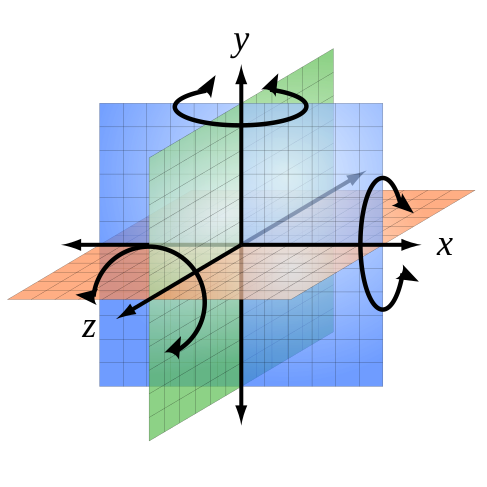
\includegraphics[width=5cm]{figs/coordinates.png}
  \end{center}
  \caption{Espacio tridimensional}
  \label{fig:espacio_tridimensional}
\end{figure}\ 

Teniendo esto en cuenta, se ha optado por usar ese número, y no uno mayor, debido a que esto encarecería los costes totales del robot, no pudiendo cumplir así 
los requisitos 1 y 5 (límite de precio y complejidad). 

Seguidamente, se debe elegir el tipo de articulación a utilizar. Aunque en robótica existen varias, en la práctica destacan dos:
\begin{itemize}
\item Revolución: Permite el movimiento de rotación alrededor de un eje fijo.
\item Prismático: Las partes del robot se pueden desplazar linealmente a lo largo de un eje específico. 

\begin{figure} [h!]
  \centering    
  \subfigure[Revolución]{\label{fig:j_rot}\includegraphics[width=0.4\linewidth ]{figs/joint_rot.png}}
  \hspace{1cm}
  \subfigure[Prismática]{\label{fig:j_prism}\includegraphics[width=0.4\linewidth]{figs/joint_prism.png}}
  \caption{Tipos de articulaciones más usadas en robótica}
\end{figure}

\end{itemize}

Finalmente, se ha optado por emplear articulaciones de tipo revolución, debido a que son más sencillas de implementar y 
están constituidas por un menor número de partes.

En cuanto a la geometría del manipulador, se debe contar con la limitación existente a la hora de tener únicamente 3 grados de libertad. Esta es 
que, aunque podemos alcanzar cualquier punto del espacio, no podemos controlar la orientación del extremo del robot en dicho punto. En base a esto, 
se ha investigado en Internet qué tipos de robot existen con ese número de grados de libertad y como lo solventan. Principalmente destacan dos 
soluciones: los robots SCARA y los robots basados en paralelogramos (presentados en la Sección \ref{sec:scara}). Ambos, tienen en común la 
característica de mantener su extremo siempre paralelo al suelo, por lo que se tiene conocimiento sobre 2 de las 3 orientaciones en ese punto. En 
la última orientación (Rotación en Z) se le suele incluir un cuarto grado de libertad, que en nuestro caso no tenemos. Aún así puede utilizarse con 
herramientas tipo electroimán o ventosas para tareas sencillas de movimiento de objetos.

Concretamente, se pretende implementar un robot basado en paralelogramos que utilice el mismo principio de funcionamiento que los utilizados en 
tareas de paletizado\footnote{Colocar objetos en un \textit{palet} de forma ordenada y eficiente}.

\section{Modelo alámbrico del manipulador}
\noindent El modelo alámbrico es una forma de analizar el movimiento de un sistema mecánico compuesto por ejes y eslabones. Este 
enfoque simplifica la representación visual al destacar las relaciones espaciales entre las diferentes partes del sistema mediante 
líneas y conexiones simbólicas.

En la Figura \ref{fig:mod_pinza_figure} se muestra un ejemplo creado específicamente para ilustrar este concepto.
\begin{figure} [ht!]
  \begin{center}
    \includegraphics[width=15cm]{figs/pinza_evol.png}
  \end{center}
  \caption{Pinza paralela con 1 grado de libertad}
  \label{fig:mod_pinza_figure}
\end{figure}\ 

A la hora de crear el modelo alámbrico de este robot, se ha tomado como referencia el del robot 
casero MeArm (Figura \ref{fig:mearm}), en concreto el modelo alámbrico usado por Juan González en la asignatura de 
Mecatrónica\footnote{\url{https://github.com/myTeachingURJC/Mecatronica/wiki/S3:-Estructuras-mec\%C3\%A1nicas-(II)}} de esta Universidad.\\
\begin{figure} [ht!]
  \begin{center}
    \includegraphics[width=15cm]{figs/mearm_params.png}
  \end{center}
  \caption{Principio fundamental del brazo MeArm}
  \label{fig:mearm_params}
\end{figure}\ 


Este robot está definido por una serie de parámetros a los que se les ha puesto nombre: L1, L2, P1, P2, P3 y A (mostrados 
en la Figura \ref{fig:mearm_params}). En función de los valores de estos parámetros, el comportamiento del brazo será diferente. Para 
encontrar los adecuados, no queda otra que utilizar la experimentación. Aún así, si se sigue un cierto orden, el proceso resulta realmente sencillo. 

\newpage
\noindent Es por esto que se ha seguido el siguiente procedimiento: 

\begin{enumerate}
\item Una manera de comenzar, es estableciendo el largo de los eslabones primarios L1 y L2. En base al tamaño de escritorio que se le pretende 
dar al robot, 17 centímetros por eslabón es un buen punto de partida.
\item El siguiente paso es elegir P1, P2 y P3. Estos son los lados cortos de los paralelogramos. Es importante jugar con estos valores 
de tal manera que se consiga obtener los más largos posibles y estos no intersecten entre sí. Esto es debido a que las piezas reales ocupan un cierto espacio y si el paralelogramo es 
muy pequeño no realizarán todo el recorrido ya que chocarán entre sí. 
\item El ángulo A restringe el paralelogramo que mantiene el extremo del robot paralelo al suelo. Este ángulo hay que variarlo ligeramente. Un buen 
punto de partida es 120º. Este valor es crítico ya que afecta significativamente a la accesibilidad del brazo a lugares próximos a su base. 
\end{enumerate}
\newpage
En la Figura \ref{fig:g_arm_alambrico} se muestra el modelo alámbrico final de este manipulador, bautizado como G-Arm\footnote{Bautizado así 
debido al lenguaje de programación que será utilizado posteriormente para comunicarse con él}:\\
\begin{figure} [ht!]
  \begin{center}
    \includegraphics[width=15cm]{figs/alambrico_garm.png}
  \end{center}
  \caption{Modelo alámbrico de G-Arm}
  \label{fig:g_arm_alambrico}
\end{figure}\ 

Dando como resultado la siguiente tabla de parámetros:
\begin{table}[H]
\begin{center}
\begin{tabular}{|c|c|}
\hline
\textbf{Parámetros} & \textbf{Valores} \\
\hline
L1 & 170mm \\
L2 & 170mm \\
P1 & 35mm \\
P2 & 35mm \\
P3 & 25mm \\
A & 135º \\
\hline
\end{tabular}
\caption{Parámetros del modelo alámbrico de G-Arm}
\label{cuadro:parametros_alambrico}
\end{center}
\end{table}
\newpage
\section{Bocetos}
\noindent Realizar bocetos es una fase clave del diseño que se lleva a cabo antes de comenzar a modelar en 3D. Con ellos, se busca tener una idea 
clara de la forma 
y posición de los elementos que constituyen el robot.  
Para el desarrollo de este brazo, se han realizado numerosos bocetos, de los cuales se conservan aquellos dibujados digitalmente en 
un iPad. En la Figura \ref{fig:bocetos} se muestran algunos de ellos.

\begin{figure} [h!]
  \centering    
  \subfigure[]{\includegraphics[width=0.5\linewidth ]{figs/boceto5.png}}
  \hspace{1cm}
  \subfigure[]{\includegraphics[width=0.4\linewidth]{figs/boceto2.png}}
  \subfigure[]{\includegraphics[width=0.4\linewidth ]{figs/boceto8.jpeg}}
  \hspace{1cm}
  \subfigure[]{\includegraphics[width=0.4\linewidth]{figs/boceto4.png}}
  \subfigure[]{\includegraphics[width=0.4\linewidth ]{figs/boceto6.jpeg}}
  \hspace{1cm}
  \subfigure[]{\includegraphics[width=0.4\linewidth]{figs/boceto7.jpeg}}
  \caption[Bocetos realizados]{}
  \label{fig:bocetos}
\end{figure}
\newpage
De hecho, antes pasar directamente al diseño \acs{CAD}, se realizó una versión en miniatura como prueba de concepto. 
Primeramente se hizo un boceto detallado en base al modelo alámbrico de la sección anterior. Posteriormente se llevó al 
ordenador para finalmente, imprimirlo en 3D. El proceso llevado a cabo, se puede ver en la \mbox{Figura \ref{fig:prueba_concepto}}.
\begin{figure} [h!]
  \centering    
  \subfigure[Boceto final]{\includegraphics[width=0.35\linewidth ]{figs/boceto1.png}}
  \hspace{2.5cm}
  \subfigure[Diseño en FreeCAD]{\includegraphics[width=0.45\linewidth]{figs/manipulador_prototipo.png}}
  \subfigure[Post-impresión]{\includegraphics[width=0.45\linewidth ]{figs/prototipo_foto2.jpeg}}
  \hspace{1cm}
  \subfigure[Tamaño del prototipo]{\includegraphics[width=0.45\linewidth]{figs/prototipo_foto1.jpg}}
  \caption[Prueba de concepto]{Evolución de la prueba de concepto}
  \label{fig:prueba_concepto}
\end{figure}

El pequeño prototipo, enteramente impreso en 3D, resultó funcional y bastante resistente, por lo que se dio por bueno el 
concepto. Gracias a haber hecho esto, se pudo tener una mejor idea de la posición de cada pieza, sirviendo de gran ayuda en 
la \mbox{Sección \ref{sec:di_cad}}.
\newpage
\section{Elección de componentes electromecánicos}
\noindent En esta sección se eligen todos aquellos componentes que no pueden ser impresos en 3D y son necesarios para 
la construcción del robot. Estos componentes deben de ser asequibles y fáciles de encontrar en páginas de Internet como 
\textit{Aliexpress} o \textit{Amazon}. Con el propósito de encontrar el conjunto ideal, se 
evaluarán diversas opciones para seleccionar aquella que ofrezca las mejores prestaciones y se ajuste al presupuesto establecido.
\subsection{Motores}
\noindent El robot requiere de 3 motores que deben contar con las siguientes características:
\begin{itemize}
  \item Capacidad de entregar suficiente torque como para levantar el brazo más la carga.
  \item Se debe poder conocer su posición en cada instante.
  \item Deben poder ejercer un torque/retención estando detenidos.
\end{itemize}

Debido a esto último, no es viable usar motores convencionales con escobillas, ya que no son 
capaces de generar torque sin girar. En cambio, los motores paso a paso si son capaces de ello. Además 
suelen disponer de una gran fuerza y, aunque no estén codificados, se puede conocer su posición angular relativa debido a que avanzan en 
pequeños incrementos discretos (pasos). Como aspecto negativo, son bastante pesados. Aún así su precio no es muy elevado por lo que es 
una opción ideal para hacer un brazo robot. 

Para estimar la fuerza necesaria, se ha realizado un análisis matemático. En la Figura \ref{fig:torque} se muestra el 
escenario de mayor esfuerzo (brazo completamente extendido) y Ecuación \ref{ec:torque} tal que da como resultado 
el torque mínimo necesario para mantener esa posición.

\begin{figure} [ht!]
  \begin{center}
    \includegraphics[width=10cm]{figs/torque.jpeg}
  \end{center}
  \caption{Dinámica del manipulador completamente extendido}
  \label{fig:torque}
\end{figure}\ 


\begin{myequation}[h!]
  \begin{equation}
    \begin{aligned}
      T1 &= m1*(L1/2) + m2*(L1 + L2/2) + payload*(L1 + L2)\\
      T2 &= m2 *(L2/2) + payload*(L1 + L2)
  \nonumber
    \end{aligned}
  \end{equation}
  \caption[Cálculo del torque necesario en la articulación más demandante]{Cálculo del torque necesario en la articulación más demandante}
  \label{ec:torque}
\end{myequation} 

Teniendo en cuenta que cada eslabón mide 17cm y se desea levantar una carga máxima de 300g, el valor de 
torque necesario en la primera articulación es y tal en la segunda.

Finalmente se ha optado por utilizar la categoría Nema 17, debido a que son comunes y fáciles de encontrar, además de tener un precio aceptable. Aunque este 
tipo de motor no es capaz de aportar por sí solo el torque necesario, más adelante se más adelante se realiza una reductora para multiplicar la fuerza 
final de dicha articulación.

\begin{figure} [ht!]
  \begin{center}
    \includegraphics[width=15cm]{figs/MotorsNema.png}
  \end{center}
  \caption{Diferentes categorías de motor paso a paso Nema \footnote{\url{https://filament2print.com/es/blog/139_motores-nema.html}}}
  \label{fig:nema}
\end{figure}\ 

Para evitar tener que hacer uso de un motor de mayor tamaño y coste, más adelante se realiza una reductora que multiplique por 5 el torque final de la 
articulación.


Dentro de la categoría Nema 17, todos tienen el mismo factor de forma a excepción del largo del motor. Esta característica determina 
el torque del motor. A mayor longitud, mayor torque es capaz de ejercer. 

Fotito de lo necesario

\newpage
\subsection{Reductora}
Para poder reducir la velocidad de giro de un motor y, a su vez convertirla en fuerza, es necesario implementar una reductora. 
Existen diferentes formas de hacerlo, como pueden ser los engranajes (normales, planetarios, helicoidales...) y las correas (lisas y 
dentadas).

Se ha optado por el uso de correas dentadas sobre el uso de engranajes, debido a que estos últimos siempre añaden una cierta holgura 
al movimiento final, haciendo el robot inexacto y añadiendo incertidumbre en los movimientos. Las correas dentadas en cambio, utilizan 
tensores para asegurar que siempre está en contacto con ambas poleas.

Foto de correa dentadas
Se pretende usar correas de tipo GT2. Este tipo de correa es ampliamente utilizado en impresoras 3D, por lo que es realmente económico y 
fácil de encontrar. Dentro de esta categoría existen diferentes anchos de correa en función de la tensión soportada. En este caso, 
se ha elegido el ancho de 6mm puesto que es el más económico con diferencia y es más que suficiente para esta aplicación.
Foto de mi correa.

Además, las poleas necesarias para este tipo de correas son fáciles de diseñar e imprimir en 3D, lo que permite hacer poleas con 
un número de dientes concreto y por un precio casi nulo.

En este caso, para dos de los grados de libertad, se ha elegido utilizar una polea comercial de 20 dientes de metal unida al 
eje del motor en conjunto con otra de 100 dientes impresa en 3D, logrando así una reducción de 1:5. En el grado de libertad restante, 
se pretende utilizar el mismo concepto pero con una polea de 120 dientes (Reducción 1:6)\footnote{Se habla de reducción 1:b cuando tal}.

\subsection{Controladores}
Debido a que se prentende utilizar motores paso a paso bipolares, es necesario utilizar un tipo de electrónica específica para 
este tipo de motor. Este componente hardware es llamado controlador, y su objetivo es convertir una señal eléctrica del controlador 
en una serie de pulsos de mayor potencia que excitarán las bobinas del motor. 
Para motores paso a paso de baja corriente (hasta 2A), existe un formato de forma común en el mundo \textit{maker}. Es por esto que la 
mayor parte de los controladores paso a paso que encontramos en el mercado son intercambiables entre sí. La diferencia entre ellos, reside 
en la tecnología de su interior y las capacidades técnicas que ofrecen. 
\begin{table}[htbp]
  \centering
  \caption{Comparación de especificaciones de los controladores existentes}
  \begin{tabular}{|c|c|c|c|c|c|}
      \hline
      \multirow{2}{*}{Modelo} & Voltaje de & Corriente & \multirow{2}{*}{Microstepping} & Nivel de & \multirow{2}{*}{Precio} \\
                             & alimentación & máxima & & ruido &\\
      \hline
      A4988 & 8-35V & 2A & Hasta 1/16 & Muy ruidoso & 1\euro \\
      \hline
      DRV8825 & 8.2-45V & 2.5A & Hasta 1/32 & Ruido aceptable & 2\euro \\
      \hline
      TMC2225 & 4.7-36V & 2A & Hasta 1/32 & Bajo ruido  & 2.8\euro \\
      \hline
      TMC2208 & 4-35V & 2A &  Hasta 1/256 & Totalmente silencioso & 2.8\euro \\
      \hline
      TMC2209 & 5.5-28V & 2.5A & Hasta 1/256 & Totalmente silencioso & 3.4\euro \\
      \hline
  \end{tabular}
\end{table}

Debido a que se pretende utilizar motores Nema 17 de más de 2A, la decisión debe estar entre el DRV8825 y el TMC2209. Finalmente, se 
ha elegido este último debido a que es realmente silencioso e incorpora una tecnología superior que garantiza una señal más definida que 
evita la pérdida de pasos del motor. Además, a la hora de adquirirlo, suele venir acompañado de un disipador de calor más grande que, unido 
a su mayor eficiencia energética, se traduce en una menor cantidad de calor dentro de nuestro robot. 

\subsection{Placa base}
La placa base es una targeta de circuito impreso que proporciona conexiones físicas y eléctricas entre las diferentes componentes y 
unifica estos en un mismo componente. 
En el caso de aquellas usadas para montar controladores paso a paso, suelen integrar un \ac{MCU} o actuar como un \textit{shield} 
(placa adicional que se acopla a otras para aumentar su funcionalidad y características).
Foto cnc arduino shield y otras

Existen numerosas opciones en el mercado con la posibilidad de montar una distinta cantidad de controladores. En el caso de este 
trabajo necesitamos sólamente 3. Este tipo de placas suelen ser utilizadas para crear máquinas CNC y en este caso se ha optado por 
elegir una placa económica que integra todo lo necesario para este proyecto a exccepción de los controladores. 
Se ha elegido esta y no otra puesto que tiene un \acs{MCU} ESP32 muy superior al AtMega328p del Arduino Uno. Además cuenta con la 
capacidad de poderse controlar vía wifi y la mayor ventaja es que incorpora un mosfet conectado a una salida pwm a la que podemos conectar 
un motor de hasta x vatios, un electroimán etc. Además incluye una serie de pines y salidas muy cónmodas de utilizar para montar 
módulos de grabado láser y etc. Todo ello por un precio de 16€.

\subsection{Fuente de alimentación}
Se trata de un elemento clave del robot. Es importante conocer \textit{a priori} las 
características necesarias de la fuente.

Por ello, se ha realizado una estimación del consumo del robot final. La mayor parte del consumo viene dado por los propios motores que 
se encontrarán permanentemente excitados con el fin de mantener el robot en una determinada posición sin desplomarse. Según las especificaciones 
de los motores escogidos, cada uno consume en torno a 7W. Es decir, el consumo de los motores es de 21W. A esto hay que añadir el consumo del 
microcontrolador y de los controladores (unos 4W). Además, si se quiere añadir un electroimán al extremo o algún servo, se necesitará de 
un extra de potencia. 
En base  a la estimación, se establece que lo ideal y recomendable para alimentar este equipo es una fuente de alimentación de 12 a 24V capaz 
de entregar al menos 30W. Si se desea usar una fuente de baja calidad, lo ideal es elegir una un 30\% más potente para evitar forzarla y aumentar 
su vida útil.
Debido al amplio rango de voltaje y de su bajo consumo, es perfectamente alimentable con un cargador típico de portátil de 19V sin temor 
a dañarlo. Pese a esto, se ha decidido utilizar una fuente de alimentacion genérica de 24V 150W para poder realizar \textit{a posteriori} 
todas las mediciones de consumos descartando a la fuente como factor limitante. El precio de esta fuente es de 15\euro.
\newpage
\subsection{Rodamientos}
Para mejorar la eficiencia de las articulaciones y garantizar que todas roten con suavidad, se pretende hacer uso de rodamientos 
en cada una de ellas. 
Existen diferentes tipos de rodamientos en el mercado pero se ha elegido un tipo de rodamiento específico para este propósito. 
Se ha optado por el uso de rodamientos brida como el de la Figura \ref{fig:rodamientos_fushi}. Este tipo de rodamientos son usados en las poleas pasivas de las impresoras 3D, por lo 
que son muy baratos (10 de buena marca por 6-10€) y sencillos de encontrar. La razón principal de su uso es su peculiar forma. Este tipo 
de rodamiento tiene un borde en el extremo que hace de borde. Esto lo hace ideal para insertar en las piezas 3D a desarrollar y garantizar 
que nunca se puedan sacar mientras el tornillo este fijado. Además evita que el rodamiento se mueva y se gire cuando la articulación 
recibe un esfuerzo lateral. (Véase la Figura \ref{fig:ejemplo_rodamiento})

\begin{figure} [ht!]
  \centering  
  \subfigure[Rodamientos F695-2RS Fushi \footnote{\url{https://es.aliexpress.com/item/32850989216.html}}]{\label{fig:rodamientos_fushi}\includegraphics[width=0.4\linewidth ]{figs/F695-2RS.jpeg}}
  \hspace{0.5cm}
  \subfigure[Ejemplo de uso]{\label{fig:ejemplo_rodamiento}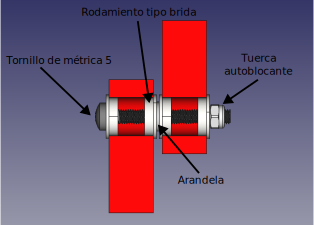
\includegraphics[width=0.5\linewidth ]{figs/RodamientosBrida.png}}
  \caption{Rodamientos de tipo brida}
\end{figure}\ 

\subsection{Finales de carrera}
Son útiles para conocer el final del recorrido de una articulación y poder establecer la posición absoluta al inicio de la 
máquina. 
Existen cantidad de ellos en el mercado y con distintas tecnologías. Se ha decidido utilizar unos basados en \textit{microswitches} debido a 
que son baratos y cumplen su función. Además son compatibles con la placa previamente elegida. 
\subsection{Electroimán}
Para realizar las pruebas, se pretende crear una herramienta para el robot que consiste en un electroimán para poder mover objetos metálicos 
de sitio. En el mercado existen muchos tipos de electroimán con distintos consumos y fuerzas. Uno ideal para esta aplicación es el \textit{D20H15}.
Su nombre indica que es un electroimán de diámetro 20mm y altura 15mm. Según las especificaciones del producto, es capaz de levantar hasta 3Kg. 
Además, es necesario comprar la versión de 24v para poder alimentarlo con tensiones entre 18 y 24v. En caso de alimentar el robot con 12v, se debería 
adquirir la versión de 12 para poder aprovechar toda su fuerza. El consumo de este electroimán es de 3W.
\newpage
\section{Diseño CAD}
\label{sec:di_cad}
\noindent En esta sección se habla de las particularidades del diseño y diversos aspectos a tener en cuenta a la hora de diseñar 
cualquier pieza mecánica que posteriormente será impresa en 3D. 
\\
Para el diseño de este brazo robot, se ha utilizado dos herramientas de diseño. Inicialmente el proyecto se realizó mediante 
la herramienta \textit{Fusion 360} y posteriormente se utilizó \textit{FreeCAD}\ref{subsec:freecad} para cumplir con el objetivo de ser totalmente 
\textit{Open Source} y estar parametrizado, para que cualquier persona pueda investigarlo, modificarlo y utilizarlo de forma gratuita.

\subsection{Base principal}
\noindent Es la parte encargada de unir el resto del robot al suelo. Dentro de ella se encuentra la placa base junto con los controladores 
y toda la electrónica a excepción de la fuente de alimentación. Esto es así debido a que puede ser alimentado de múltiples formas (baterías, 
cargadores de ordenador, fuentes de PC, salidas de alimentación de robots móviles, etc). Además, esta electrónica debe poder estar refrigerada 
por un pequeño ventilador incorporado en la propia base. \\
Se optó por realizar dos piezas circulares y una serie de espaciadores anchos que unían el conjunto, dejando espacio en el interior para 
la placa base. Este tipo de piezas son muy robustas y fáciles de imprimir. 
\begin{figure} [ht!]
  \begin{center}
    \includegraphics[width=12cm]{figs/base_principal.png}
  \end{center}
  \caption{Base principal}
\end{figure}\ 

\subsubsection{Pieza circular superior}
\noindent La pieza circular superior (Figura \ref{fig:base_principal_superior}), incluye una serie de agujeros y huecos hexgonales para insertar las tuercas M3 que permiten
acoplar la polea de 120 dientes (Figura \ref{fig:base_principal_polea}). Además, incluye un rebaje de 40mm en un lateral para poder insertar y atornillar un ventilador 4010.
\subsubsection{Espaciadores}
\noindent Los espaciadores (Figura \ref{fig:base_principal_espaciadores}) constan de 4 cilindros perforados con un agujero de 5mm por el que entrarán los tornillos de métrica 5.
\subsubsection{Pieza circular inferior}
\noindent La pieza circular inferior (Figura \ref{fig:base_principal_inferior}), contiene una serie de agujeros para poder atornillar la placa base. Además contiene una serie de agujeros en su perímetro 
para poder atornillar el robot al suelo. 

\begin{figure} [ht!]
  \centering    
  \subfigure[Polea 120 dientes]{\label{fig:base_principal_polea}\includegraphics[width=0.45\linewidth ]{figs/base_principal_polea.png}}
  \hspace{1cm}
  \subfigure[Pieza superior]{\label{fig:base_principal_superior}\includegraphics[width=0.45\linewidth]{figs/base_principal_superior.png}}

  \subfigure[Espaciadores]{\label{fig:base_principal_espaciadores}\includegraphics[width=0.45\linewidth]{figs/base_principal_espaciadores.png}}
  \hspace{1cm}
  \subfigure[Pieza inferior]{\label{fig:base_principal_inferior}\includegraphics[width=0.45\linewidth]{figs/base_principal_inferior.png}}
\end{figure}
\newpage
\subsection{Base de los motores}
\noindent Este conjunto es el encargado de contener los 3 motores y rotar sobre la base principal.
\begin{figure} [ht!]
  \begin{center}
    \includegraphics[width=12cm]{figs/base_motores.png}
  \end{center}
  \caption{Base de los motores}
\end{figure}\ 
\\
Consiste principalmente en 4 piezas; las dos laterales, la inferior y un espaciador de lado a lado que refuerza el conjunto. Esta ideado así 
para realizar piezas que serán imprimidas en dirección horizontal que es como mayor resistencia tienen las piezas en impresora 3d por la 
dirección de las capas. Además se consigue la máxima exactitud en los orificios y formas circulares. Todo el conjunto se une a través de 
varillas roscadas y tuercas.

Cabe recalcar el sistema de tensado de las correas. Consiste en una serie de orificios longitulidanes y una pieza que agarra el motor por 
el otro lado a modo de sandwich.
foto de lateral que se vea eso

Además esta pieza incorpora 2 de los 3 finales de carrera del robot. Además tiene una serie de ranueras para poder poner bridas a posteriori y 
organizar bien los cables.
\newpage
\subsection{Paralelogramos}
\newpage
\subsection{Elemento terminal}
\noindent Esta pieza (Figura \ref{fig:extremo_pieza}) está la situada en el extremo del robot. Es la encargada de realizar la unión entre el robot y la herramienta. Por esto, 
se ha ideado con una forma particular que permite acoplar herramientas de una forma sólida e inequívoca. 
\begin{figure} [ht!]
  \begin{center}
    \includegraphics[width=10cm]{figs/extremo_robot.png}
  \end{center}
  \caption{Elemento terminal}
  \label{fig:extremo_pieza}
\end{figure}\ 
\\
Consiste en una acanaladura a 45 grados (Figura \ref{fig:vistas_extremo}) con un agujero que la atraviesa, por el que pasará el tornillo unirá ambas piezas. 
Este acople, diseñado específicamente para este proyecto, es sencillo de usar e impide que la herramienta rote o 
tenga algún tipo de holgura. De hecho, las paredes están en ángulo para obligar a la herramienta a centrarse en la acanaladura y hacer 
la unión muy robusta y precisa.
\begin{figure} [ht!]
  \begin{center}
    \includegraphics[width=14cm]{figs/vistas_extremo.png}
  \end{center}
  \caption{Vistas del elemento terminal}
  \label{fig:vistas_extremo}
\end{figure}\ 

\subsection{Herramienta electroimán}
\noindent Para dotar al robot de una utilidad, se ha creado una herramienta que contiene el electroimán (Figura \ref{fig:electroiman_pieza}). Esta herramienta debe de tener la forma 
de la acanaladura anterior para poder encajar en el robot. Además se ha redondeado las esquinas para que visualmente se adapte mejor a la 
forma del extremo del robot. Para unir el conjunto se ha utilizado el propio orificio roscado del electroimán, como se puede ver en la Figura 
\ref{fig:electroiman_montaje}

\begin{figure} [ht!]
  \centering    
  \subfigure[Pieza]{\label{fig:electroiman_pieza}\includegraphics[width=0.8\linewidth ]{figs/electroiman_solo.png}}

  \subfigure[Montaje]{\label{fig:electroiman_montaje}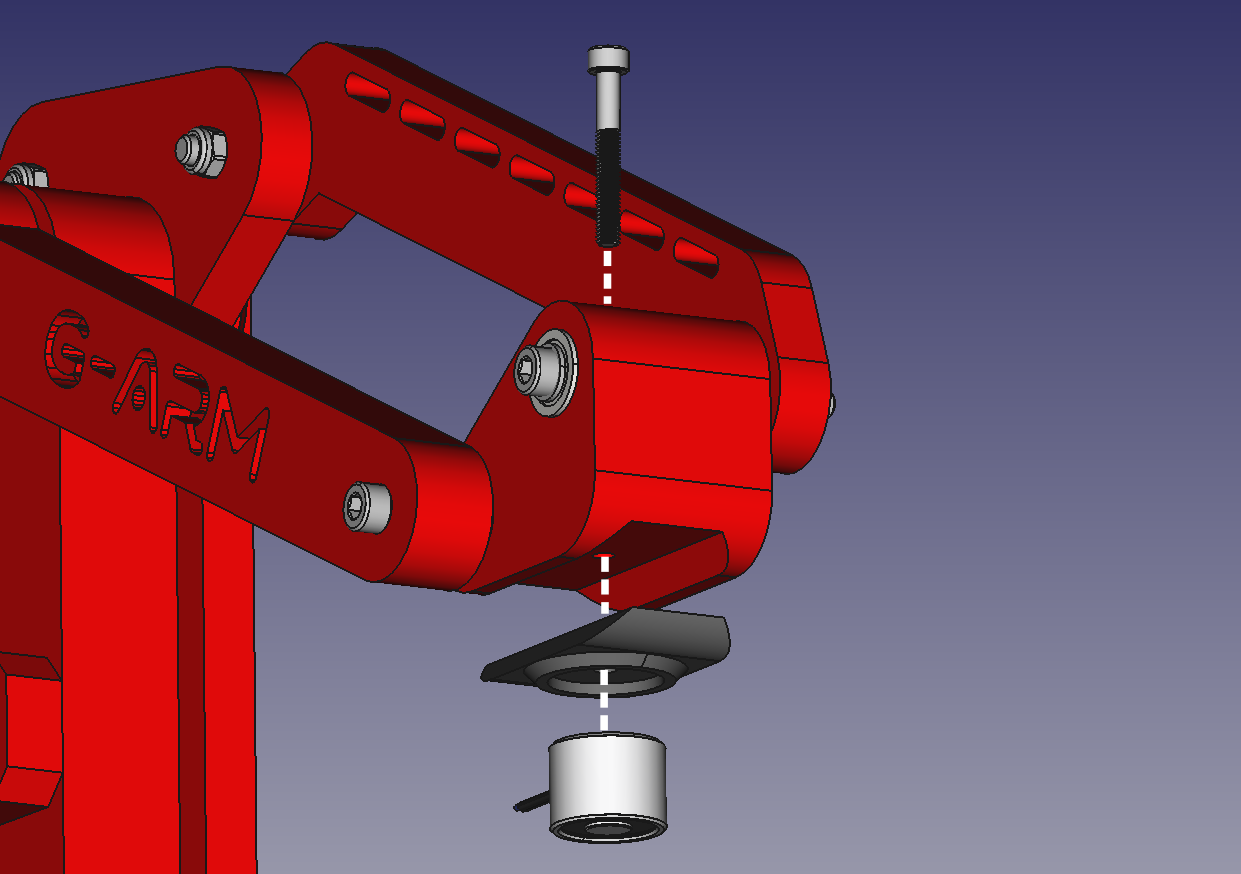
\includegraphics[width=0.8\linewidth]{figs/electroiman_montaje.png}}
  
  \caption{Herramienta electroimán}
\end{figure}

\newpage
\subsubsection{Diseño de las poleas dentadas}
Primero, se ha utilizado la herramienta \textit{online} 
gt2-gear-generator\footnote{\url{https://avtehnik.github.io/gt2-gear-genaretor/}} para generar de manera paramétrica el contorno de la polea 
en formato DXF.\\
\begin{figure} [ht!]
  \begin{center}
    \includegraphics[width=14cm]{figs/dxf_polea.png}
  \end{center}
  \caption{Contorno de la polea de 100 dientes}
\end{figure}\ 
Posteriormente, abrimos el fichero DXF mediante el \textit{workbench} Draft de FreeCad y seleccionamos todos los contornos. A continuación, 
pulsamos en el icono de "Borrador a Croquis" de la barra superior de herramientas y se nos generará un boceto de FreeCad que podremos extruir 
con el \textit{workbench} Part Design. 
\begin{figure} [ht!]
  \begin{center}
    \includegraphics[width=1cm]{figs/polea_freecad.png}
  \end{center}
  \caption{Contorno de la polea de extruido}
\end{figure}\ 

\subsubsection{Mecanismo de tensado de la correa}


\newpage
\section{Impresión y montaje}
\noindent En esta sección se exponen todos los detalles a tener en cuenta a la hora de querer replicar este proyecto. Para la impresión 
de G-Arm se ha utilizado una impresora Ender-3 Pro\footnote{\url{https://www.creality.com/products/ender-3-pro-3d-printer}} y un rollo 
de 1Kg de filamento PLA Rojo convencional.
\begin{figure} [h!]
\begin{center}
  \includegraphics[width=8cm]{figs/ender3.png}
\end{center}
\caption{Ender-3 Pro V1 2017}
\label{fig:ender3pro}
\end{figure}\   

Con la intención de lograr la mejor organización posible, se ha decidido incluir una serie de tablas 
detallando los componentes necesarios para el montaje del robot. En la Tabla \ref{cuadro:componentes} se listan aquellos 
componentes que deben ser comprados y su precio. Se recomienda adquirirlos a través de páginas como \textit{Aliexpress} ya que 
resulta significativamente más barato que comprarlos a través de \textit{Amazon}. Por otro lado, es necesaria la tornillería 
de la Tabla \ref{cuadro:tornilleria}, comprada en ferreterías locales y nacionales como \textit{Randrade} (Online). El resto 
de piezas detalladas en la Tabla \ref{cuadro:piezas}, son enteramente imprimibles en 3D. Se recomienda configurar el laminador 
con las densidades de relleno propuestas en dicha tabla. Cada pieza está diferenciada con un número y se pueden requerir varias 
unidades de una misma pieza (indicado en la propia tabla).
\begin{table}[H]
\begin{center}
\begin{tabular}{|c|c|c|c|}
\hline
\textbf{Componente} & \textbf{Modelo} & \textbf{Cantidad} & \textbf{Precio total} \\
\hline
Motor Nema 17 & 17HS24-2104S & 3 & 56\euro \\
Controlador & TMC2209 & 3 & 10\euro \\
Placa base & MKS DLC32 & 1 & 16\euro \\
Final de carrera & MakerBot (rojo) & 3 & 5\euro \\
Fuente de alimentación & 24V 5A (opcional)\ref{subsec:fuente_alimentacion} & 1 & 15\euro \\
Rodamiento &  F695-2RS Fushi & 22 & 15\euro \\
Rodamiento & F623RS Fushi & 6 & 5.5\euro \\
Polea GT2 & Correa:6mm ID:5mm & 3 & 1.5\euro \\
Correa GT2 & Correa:6mm Largo:252mm & 2 & 3.5\euro \\ 
Correa GT2 &  Correa:6mm Largo:280mm & 1 & 1.8\euro \\ 
Ventilador & 24V 4010 & 1 & 2\euro \\
Electroimán & D20H15mm 3KG 24V & 1 & 3\euro \\
Plástico para imprimir & PLA/PETG 1Kg & 1 & 22\euro \\
\hline
\end{tabular}
\caption{Componentes hardware necesarios}
\label{cuadro:componentes}
\end{center}
\end{table}

\begin{table}[H]
\begin{center}
\begin{tabular}{|c|c|c|}
\hline
\textbf{Componente} & \textbf{Cantidad} & \textbf{Precio total} \\
\hline
Tornillo M3 Allen & 3 & 56\euro \\

\hline
\end{tabular}
\caption{Tornillería necesaria}
\label{cuadro:tornilleria}
\end{center}
\end{table}


\begin{table}[H]
\begin{center}
\begin{tabular}{|c|c|c|}
\hline
\textbf{Identificador} & \textbf{Cantidad} & \textbf{Relleno óptimo} \\
\hline
\#1 & 1 & 15\% \\
\hline
\end{tabular}
\caption{Piezas necesarias}
\label{cuadro:piezas}
\end{center}
\end{table}

El precio total de los componentes necesarios es de 156.3\euro sumado a los tantos de tornillería, hacen un coste total de tanto.\\

La impresión de todas las piezas (utilizando una altura de capa de 0.12mm) puede llevar cerca de 60 horas. En cambio, 
el montaje requiere de apenas 2, o incluso, menos dependiendo de la habilidad del usuario. Para saber la posición de cada pieza 
y dónde montarla, se recomienda consultar el montaje 
completo\footnote{\url{https://github.com/RoboticsURJC/tfg-vperez/blob/280861172bce3b1c0cfbb155a434364ea68eeb30/src/design/FreeCad/\%230\_ASSEMBLY.FCStd}} 
realizado mediante A2Plus en FreeCAD. En él, se puede ver 
el nombre de cada pieza, tornillo necesario y posición.
\\

En cuanto al montaje de la electrónica es realmente sencillo debido a que existen numerosos tutoriales 
y manuales en internet que utilizan esta placa. Por si no fuera poco, el propio circuito impreso de la 
placa tiene serigrafiado un nombre en cada conector. El unico aspecto a tener en cuenta es la regulación 
de corriente de los 3 controladores TMC2209. Esta se realiza mediante un pequeño potenciómetro y requiere 
de un multímetro para leer los valores. En este \href{https://all3dp.com/2/vref-calculator-tmc2209-tmc2208-a4988/}{enlace} se muestra un tutorial de como hacerlo.

\clearpage
\thispagestyle{empty}

\printindex \nocite{*}
\appendix
\bibliographystyle{apalike} \bibliography{bibliografia}

\end{document}
